\documentclass{my_paper}
\usepackage{ctex}
\usepackage[textwidth=444bp,vmargin=2.5cm]{geometry}%设置页边距
\usepackage{array} %主要是增加列样式选项
\usepackage[dvipsnames]{xcolor}%颜色宏包
\usepackage{graphicx}%图片宏包
\usepackage{amsmath}%公式宏包
\usepackage[T1]{fontenc}    
\usepackage{newtxtext, newtxmath}  %两种使用Times New Roman 字体的方法
\usepackage{subfigure}
\usepackage{tabularx, booktabs} %% Load packages that you use
\usepackage{multirow} %跨行处理
\usepackage{rotating}%横向表格
\usepackage{diagbox}%斜线划分表头

\usepackage { gensymb }
% 打°符号\degree
\usepackage{framed}
\usepackage{listings}
% 代码
\usepackage{color} %red, green, blue, yellow, cyan, magenta, black, white
\usepackage[numbered,framed]{matlab-prettifier}%matlab 代码高亮
\usepackage{mdframed}%另一个边框
% matlab代码样式,使用方法为:
% \lstinputlisting[style=Matlab-editor,linewidth=\textwidth]{code.m}
% 或:
% \begin{lstlisting}[style=matlab-prettifier]
%     %code
% \end{lstlisting}
\begin{document}

\lstdefinestyle{python_style}{
 columns=fixed,
 numbers=left,                                        % 在左侧显示行号
 numberstyle=\tiny\color{gray},                       % 设定行号格式
 frame=trbl,                                        % 单线背景边框
 breaklines=true,                                     % 设定LaTeX对过长的代码行进行自动换行
 keywordstyle=\color[RGB]{40,40,255},                 % 设定关键字颜色
 numberstyle=\footnotesize\color{darkgray},
 commentstyle=\it\color[RGB]{0,96,96},                % 设置代码注释的格式
 stringstyle=\rmfamily\slshape\color[RGB]{128,0,0},   % 设置字符串格式
 showstringspaces=false,                              % 不显示字符串中的空格
 language=python,                                        % 设置语言
 basicstyle=\linespread{1.0}\fontsize{10bp}{10bp}\selectfont\ttfamily,                      % 字体字号
 %lineskip=10bp,
 %baselinestretch=1,
}
\newpage
\begin{center}
\lunwenbiaoti

\vspace{2ex}
\zhaiyao
\end{center}

摘要

\begin{guanjianci}
 元胞自动机 \quad 边缘检测 \quad 形状匹配
\end{guanjianci}

%----------- 正文 ----------
%----------- 一、问题重述 ----------
\newpage
\section{一、问题重述}

暖气在我国北方地区被广泛使用,在寒冷的气候条件下,暖气可以调节室内温度,带来舒适的室内环境。在使用暖气的过程中,人们常常希望把温度控制在舒适的范围内。因此如何通过控制供热水流的大小来调节室内温度成为广大研究者关注的问题。

一种智能温控器被用于完成调节温度的任务。这一工具具有调节流量的作用,可以主动调节水流大小,以满足升高温度的需求,对于降低温度而言,只能关闭阀门留待暖气片中的水流自然冷却,温度回落到室温。该装置存在温度调节不智能,过度加热或冷却,温度波动变化大的缺点。

经过分析整理,我们需要解决以下问题:
\begin{enumerate}
    \item 分析一个房间的采暖过程中的热量从供热管道到加热房间的过程,并建立模型来描述供热的水温与热水流量与房间内温度的关系。
    \item 在给定波动的室外温度条件下,针对室内某个位置设定的目标温度,设计对供热水流的调节方法。以尽可能少的次数来调节水流大小,使得室内温度最快达到目标温度。并利用附件中的数据给出控制的结果,说明方法的合理性。
    \item 假设温度控制器能记录下过去的调节结果,比如室外温度,用户设定温度,供热水阀门开闭程度,热水温度等。房间大小、房间中的属性、封闭程度、墙窗门的比例、墙壁保温程度等相对固定的。在上述条件下,对第二问中的控制方法进行优化。
\end{enumerate}

\section{二、问题分析}
\subsection{问题一的分析}

问题一我们需要分析房间采暖过程的热量转移过程,要求我们就暖气这一供热装置的原理有所了解。为此需要查阅资料与相关参数,分析暖气片的热交换方式,以及分析进水温度$T_{wi}$和出水温度$ T_{wo} $与热量传递$Q$之间的关系。为了建立模型,描述供热水温与热水流量同房间内温度的关系问题,需要就房间的整体结构进行分析。房间由墙体,窗户,以及天花板构成,部分墙体属于外墙与室外相接触,而有的墙体又属于内墙,内外墙之间的传热能量具有差异。此外,考虑空气导热性质不佳的特点,需要结合传热学知识,建立全屋的空气热量模型。

\subsection{问题二的分析}

分析

\subsection{问题三的分析}


%----------- 三、模型假设 ----------
\section{三、模型假设}
%使用代码片段:、jiashe%
\begin{enumerate}
    \item 
    
    \textbf{原因:}


\end{enumerate}

%----------- 四、符号说明 ----------
\section{四、名词解释与符号说明}
%使用三线表格最好~
\subsection{名词解释}
\begin{enumerate}
    % 名词:、mingci
    \item \textbf{dada}
    
    dsadw
    
    \item \textbf{dsadc}
    
    dasdsas

    
\end{enumerate}
\subsection{符号说明}
以下是本文使用的符号以及含义:
\begin{table}[h]%htbp表示的意思是latex会尽量满足排在前面的浮动格式,就是h-t-b-p这个顺序,让排版的效果尽量好。
    \centering
    \begin{tabular}{p{2.0cm}<{\centering}p{9.0cm}<{\centering}p{2.0cm}<{\centering}}
 %指定单元格宽度, 并且水平居中。
    \hline
    符号 & 说明 & 单位 \\ %换行 
    \hline
    $L_0$ & 仓库长度 &  $m$\\
    
    \hline
    \end{tabular}
\end{table}

%----------- 五、模型的建立与求解 ----------
\section{五、模型的建立与求解}

以下将对提出的三个问题进行建模求解。
\subsection{热水调控的房间温度模型}

为了解决问题一,我们提出一种以房间热水流量和热水温度为输入,以最终房屋每处温度随时间的变化为输出的模型。为此,我们对暖气片的工作原理,房间的结构和传热特性进行分析。在得到房屋的热量传递模型后,结合牛顿冷却定律、傅里叶传热定律以及热量守恒定律,建立离散化的屋内温度模型。

\subsubsection{暖气片供热模型}

暖气片利用热水在管中流动的过程,加热其周围的空气,并传递热量到周围,是一种典型的间壁式散热器\cite{2}。在工作过程中,暖气片的热水从一端流入,并且从另一端流出较冷的水,在内部为相连的若干U形管相连,如 图(\ref{nuanqipian})所示:

\begin {figure}[h]
\centering % 居中显示
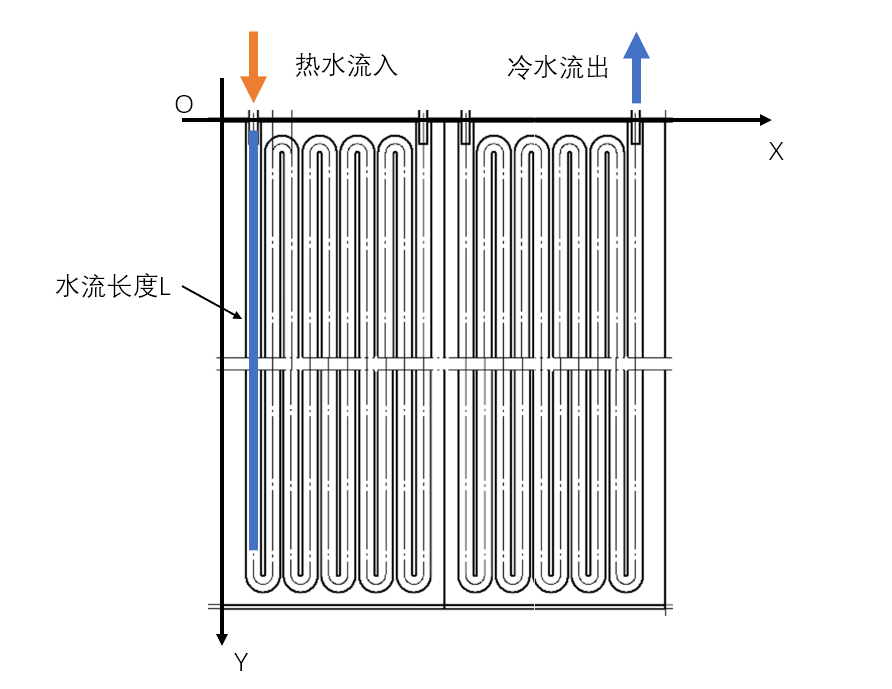
\includegraphics[width=\textwidth]{nuanqipian.png}
说明:为展示方便,z轴垂直纸面向内,隐去不画。
\caption{暖气片内部水流示意图} % 标题
\label{nuanqipian}
\end {figure}

在$ t=0 $时,热水还未流入管内,此时管内水流温度等于室内温度$ T_{s0} $;

在经过时间 $t_0$ 后,热水流入管中,此时管中热水长度$l$为:

\begin{equation}
l_0 = \int^{t_0}_{0}\frac{v(t)}{S}dt
\end{equation}

其中$ v(t) $为热水流量,随调节过程随时间变化,$ S $为暖气管的横截面积。在水流长度为$ l $的情况下,对应在图(\ref{nuanqipian})中的直角坐标系,有唯一的坐标表示$(x,y,z)=f(l)$,即:

\begin{equation}
\begin{cases}
    x = f_x(l)\\
    y = f_y(l)\\
    z = f_z(l)\\
\end{cases}
\end{equation}

取时间微元$ t\to t+dt $进行分析,此时长度变化为$dl$,使用水流速度$v(t)$,横截面积$S$计算而出。

\begin{equation}
    dl = \frac{v(t)*dt}{S}
\end{equation}

考虑该段微元处的管道导热影响,我们画出其截面图(图\ref{jiemian}),对于该段柱体而言,可以假设管内的温度为$T_1$而管外温度为$T_2$,观察暖气管的物理结构可知,满足长度远远大于其直径,可以看作是等温面共轴。在这一条件下,建立热传导微分方程:

\begin{equation}
\frac{d^{2}T}{dr^{2}} + \frac{1}{r}\frac{dT}{dr}
\end{equation}

使用变量代换法,将上式变形:
\begin{equation}
u = \frac{dT}{dr} \Rightarrow  \frac{du}{dr}=\frac{d^2T}{dr^2}
\label{}
\end{equation}

之后将原始微分方程变化为以下形式:
\begin{equation}
\frac{du}{dr}+\frac{u}{r} = 0
\label{}
\end{equation}

可以通过分离变量法和两部积分法,可以求出对数形式的同届:
\begin{equation}
    \begin{cases}
        ln u +lnr = lnC_1\\
        T(r) = C_1 lnr + C_2
    \end{cases}
\label{}
\end{equation}

通过给定第一类边界条件\cite{1},即表面温度分布,如下所示:
\begin{equation}
    \begin{cases}
        r = r_1 , & T = T_1\\
        r = r_2 , & T = T_2
    \end{cases}
\end{equation}

可以计算出柱体内的最终温度场形式:
\begin{equation}
    T(r) = T_1 - (T_1-T_2)\frac{lnr - lnr_1}{lnr_2 - lnr_1}
\end{equation}

利用傅里叶传热定律计算出表面的热流密度$\phi$:

\begin{equation}
    \phi = -\lambda \frac{dT}{dr} = \frac{\lambda}{r}\frac{T_1-T_2}{lnr_1-lnr_2}
\end{equation}

经过上述分析,我们建立了水流经由暖气管向外散发热量的过程,在完成上述过程后分析一段微元$dl$处的热交换情况。由于微元处的长度很小,该段微元的温度可以由微元开始处的温度$T_n(l,t_0)$所确定。我们利用牛顿冷却定律\cite{1},在水柱微元和空气之间建立如下所示的传热关系:

\begin{equation}
    \begin{aligned}
        q&= k_0*(T(x,y,z,t_0)-T_n(l,t_0))\\
        &= k_0 * (T(f_x(l),f_y(l),f_z(l),t_0)-T_n(l,t_0))
    \end{aligned}
\end{equation}

其中$T,T_n$分别代表室内空气温度和暖气温度,$q$代表热流密度,含义是单位时间内单位面积处发出或接受的热量。我们利用$ q $可以求得一段水柱微元内的热量变化$dQ$,以及由于热量变化所导致的温度变化$dT_n$:
\begin{equation}
    dQ = q* C * dl * dt
\end{equation}

$q$代表热流密度,$C$为暖气管的截面周长,又依据比热容的计算公式,算出一段水柱的温度变化:
\begin{equation}
    dT_n(l,t_0) = \frac{dQ}{c*s*dl*\rho}
    \label{dt}
\end{equation}

在这里$c$代表水的比热容,$S$代表管道截面积。由于水管中水流不断移动,相邻两段微元之间的温度差很小,近似认为不发生热交换,故在我们的模型中,该暖水微元的温度变化数值$dT$为后一时刻的同一段水柱温度变化,因此式(\ref{dt})被解释为:
\begin{equation}
dT_n(l,t_0) = T_n(l+dl,t_0+dt) - T_n(l,t_0)
\label{}
\end{equation}

也就是说在$ dt $的时间间隔内,暖水微元移动了$dl$距离,但是在分析温差变化时,还是计算同一段水柱的变化数值。至此,我们已经阐述了流水在暖气管道中的热交换问题,在下面的内容中,我们将同样使用微分的方法,以能量守恒定律,牛顿冷却定律,傅里叶传热定律建立屋内空气变化模型。



\section{六、敏感性分析}
\section{七、模型的评价}

\subsection{模型的优点}
\begin{enumerate}
    \item 采用

\end{enumerate}

\subsection{模型的缺点}
\begin{itemize}
    \item 利用较

\end{itemize}

%----------- 参考文献 ----------
\newpage
\bibliographystyle{unsrt} %规定了参考文献的格式
\begin{center}
\bibliography{reference} %调出LaTeX生成参考文献列表
\end{center}

%----------- 附录 ----------
\newpage
\section{附件}
\textbf{附件清单:}
\renewcommand\theenumi{\roman{enumi}}
% 规定数字格式为罗马数字
\renewcommand\labelenumi{\textbf{附录\theenumi}}
% 规定是附录某某
\begin{itemize}
    \item xxx代码
\end{itemize}

\textbf{sobel边缘检测代码}

\begin{lstlisting}[language=matlab]
    function GAdsa 
\end{lstlisting}



\end{document}